\documentclass[dvipsnames, svgnames, x11names, 11pt]{article}

\usepackage[paper=a4paper, top=2cm, bottom=3cm, right=2.6cm, left=2.6cm]{geometry}

\usepackage{xcolor}
% URLs and hyperlinks 
\usepackage{hyperref}
\hypersetup{
    colorlinks=true,
    linkcolor=DarkBlue,
    filecolor=magenta,
    urlcolor=blue,
}
\usepackage{xurl}
%

\usepackage{amsmath, mathtools}
\usepackage{footnotehyper}
\usepackage{multirow}
\usepackage{longtable}
\usepackage{float}
\usepackage{paralist}
\usepackage{graphicx}
\renewcommand{\arraystretch}{1.23}

\newcounter{secq}
\setcounter{secq}{0}
\newcommand{\seccnt}{\stepcounter{secq}\arabic{secq}. }

\newcounter{swotq}[secq]
\setcounter{swotq}{0}
\newcommand{\swotqcnt}{\stepcounter{swotq}\arabic{secq}.\arabic{swotq}. }

\usepackage{xepersian}
\settextfont{Yas}
\setdigitfont{Yas}

\title{فاز دوم پروژه}
\author{
محدثه آخوندی \\
مهدی حق‌وردی \\
سعید رنجبر
}
\date{}

\begin{document}
\maketitle
\tableofcontents
\listoffigures

\section{خلاصه مدیریتی}
مدیریت در سوبریو به دو بخش 
\begin{inparaitem}
\item 
مدیریت تیم کسب و کار
\item 
مدیریت تیم توسعه
\end{inparaitem}
تقسیم می‌شود.

این جداسازی به این دلیل است که ساختار کاری سوبریو پر از کارمندان و مشاورانی است که در ارتباط مستقیم با مشتری هستند و ارگان‌های زیادی با ما همکاری دارند. پس برای مدیریت بهتر و آسان‌تر بهتر است که تیم کسب و کار از تیم توسعه جدا شوند.

\subsection{مدیریت تیم کسب و کار}
برای تیم کسب و کار ما از ساختار سازمانی مسطح
\lr{(Flat Organizational Structure)}
استفاده می‌کنیم. 

ساختار سازمانی مسطح (یا ساختار سازمانی افقی) با سطح مدیریتی محدود بین رهبری عالی کسب و کار و کارمندان سطح پایین‌تر است. کارمندان ممکن است مستقیماً به صاحب کسب و کار یا فقط به یک یا دو سطح مدیریت که برای همه تیم نظارت دارند پاسخ دهنده باشند.

ویژگی‌های این ساختار

\begin{itemize}
\item 
لایه‌های مدیریتی کمتر 

در این ساختار لایه‌های مدیریتی خیلی کمتری نسبت به ساختار عمودی وجود دارد و تعامل بین کارمندان و مدیران بسیار بیشتر و سازنده‌تر است.

\item 
انعطاف‌پذیری و سازگارپذیری بیشتر

سازمان‌های مسطح معمولاً با تغییرات سازگارتر هستند. فقدان سطوح سلسله مراتبی گسترده به آنها اجازه می دهد تا سریعتر به تغییرات بازار یا محیطی واکنش نشان دهند.

\item 
محیط کاری خودمانی

سازمان‌هایی با این ساختار تمایل دارند محیط کاری غیررسمی و آرام‌تری را ایجاد کنند. نزدیکی کارکنان به مدیریت ارشد و کاهش تاکید بر عناوین رسمی به ایجاد فضایی نزدیک‌تر و دوری از محیطی خشک و آشفته کمک می‌کند.

\item 
سبک رهبری مربیگری

رهبران در سازمان‌های مسطح معمولاً یک سبک مربیگری را به جای سبک خودکامه اتخاذ می‌کنند. این رویکرد با تأکید بر توانمندسازی و مشارکت کارکنان است.
\end{itemize}

\subsubsection{شمای ساختار مدیریتی}
\begin{figure}[H]
\begin{center}
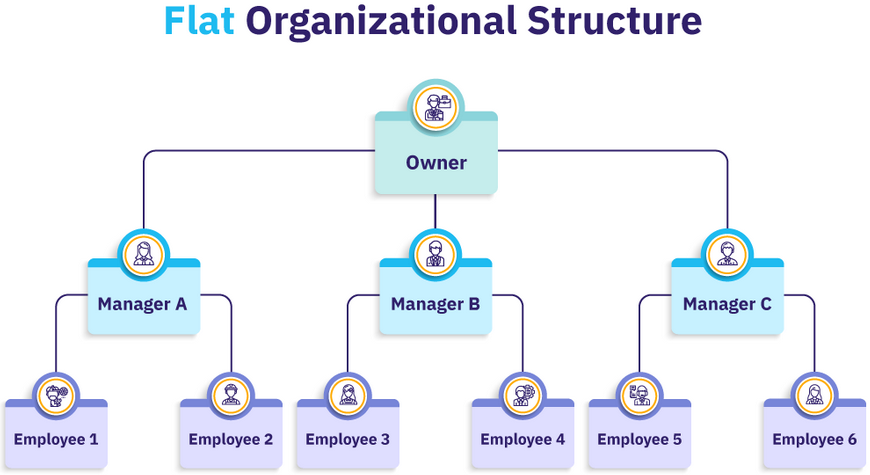
\includegraphics[scale=0.5]{../images/flat}
\end{center}
\caption{شمای ساختار مدیریتی}
\end{figure}

مدیریت این تیم توسط
\lr{CEO}
انجام می‌گیرد و مدیران میانی توسط ایشان انتخاب می‌شوند.

\subsection{مدیریت تیم توسعه}
از سوی دیگر مدیریت تیم توسعه توسط 
\lr{CTO}
انجام می‌شود و تمامی تصمیمات تخصصی و 
\lr{technical}
توسط ایشان گرفته می‌شوند. مدیریت تیم‌لید‌های تیم‌های مختلف هم به عهده‌ی ایشان است. 

تصمیمات و سیاست‌های کسب و کار توسط 
\lr{CEO}
به ایشان گفته می‌شوند و تسک‌های اسپرینت‌های مختلف با نظر ایشان ایجاد و تقسیم می‌شوند.

توسعه در این تیم به صورت 
\lr{scrum}
مدیریت و انجام می‌شود و 
\lr{scrum master}
مسئول هماهنگی بین تیم‌ها و 
\lr{CTO}
است.

در واقع ساختار مدیریت این تیم هم کاملا افقی‌ست. یک مدیر
\lr{CTO}
یک اسکرام مستر و چندین تیم توسعه.

\section{ساختار تیم مورد نیاز جهت پیاده‌سازی کسب و کار}
\subsection{معرفی تیم}
تیم سوبریو، همانطور که بالاتر هم اشاره شد به دو بخش \textit{تیم کسب و کار} و تیم \textit{توسعه} تقسیم می‌شود. 

از آنجایی که سوبریو به دو بخش بزرگ \textbf{پیشگیری و آموزش} و \textbf{رهاسازی} تقسیم می‌شود به دو مدیر ارشد برای هر کدام از این بخش‌ها برای مدیریت نیاز پیدا کرده است.

\begin{itemize}
\item \textbf{مدیر بخش رهاسازی}: آقای سعید رنجبر،
\item \textbf{مدیر بخش پیشگیری و آموزش}: سرکار خانم محدثه آخوندی و
\item \textbf{مدیر تیم توسعه}: مهدی حق‌وردی
\end{itemize}

مدیریت کل کسب و کار سوبریو هم توسط برد اجرایی که شامل ما سه نفر است انجام می‌شود و تصمیمات با رای اکثریت از بین ما سه نفر اتخاذ می‌شود.

\subsection{چرا تیم فعلی می‌تواند برنده باشد}
به چه دلایلی تیم ما می‌تواند موفق باشد
\begin{itemize}
\item 
درک عمیق از مشکل

تیم سازنده به نظر می‌رسد درک عمیقی از مشکل اعتیاد و چالش‌های مرتبط با آن دارد. این درک عمیق منجر به طراحی یک راهکار جامع شده که نیازهای مختلف افراد درگیر با اعتیاد را پوشش می‌دهد.

\item 
رویکرد چندجانبه

ین بوم کسب‌وکار یک رویکرد چندجانبه را برای مبارزه با اعتیاد اتخاذ کرده است. از پیشگیری و آموزش تا درمان و حمایت، تمام جوانب این مشکل در نظر گرفته شده است.


\item 
استفاده از فناوری

استفاده از فناوری‌های نوین مانند هوش مصنوعی و یادگیری ماشین برای شخصی‌سازی محتوا و ارائه خدمات، می‌تواند به بهبود اثربخشی این پلتفرم کمک کند.

\item 
مدل کسب‌وکار متنوع

مدل کسب‌وکار این پلتفرم ترکیبی از منابع درآمدی مختلف مانند اشتراک‌های پرمیوم، همکاری با سازمان‌های دولتی و خصوصی و حمایت‌های مالی خیرین است که می‌تواند به پایداری مالی آن کمک کند.

\item
تیم مدیریتی قوی

وجود سه مدیر ارشد با تخصص‌های مختلف و رویکرد مشارکتی در تصمیم‌گیری، نشان از یک تیم مدیریتی قوی و کارآمد دارد.
\end{itemize}

اما در ادامه فاکتور‌های دیگری که به موفقیت یا شکست کسب و کار منجر خواهند شد عبارتند از
\begin{inparaitem}
\item 
تیم فنی،
\item 
استفاده درست از بازار هدف،
\item 
داشتن مزیت رقابتی و مدیریت کردن رقبا و
\item 
منابع مالی.
\end{inparaitem}
اگر این مسائل به درستی مدیریت شوند می‌توان گفت که در مدت معقولی کسب و کار به نقطه‌س سر به سر و سپس رشد می‌رسد.

\section{اطلاعات کسب و کار}

\subsection{مدل کسب و کار}
مدل کسب و کار در تصویر
\ref{fig:canvas}
آورده شده است.

\begin{figure}[b]
\begin{center}
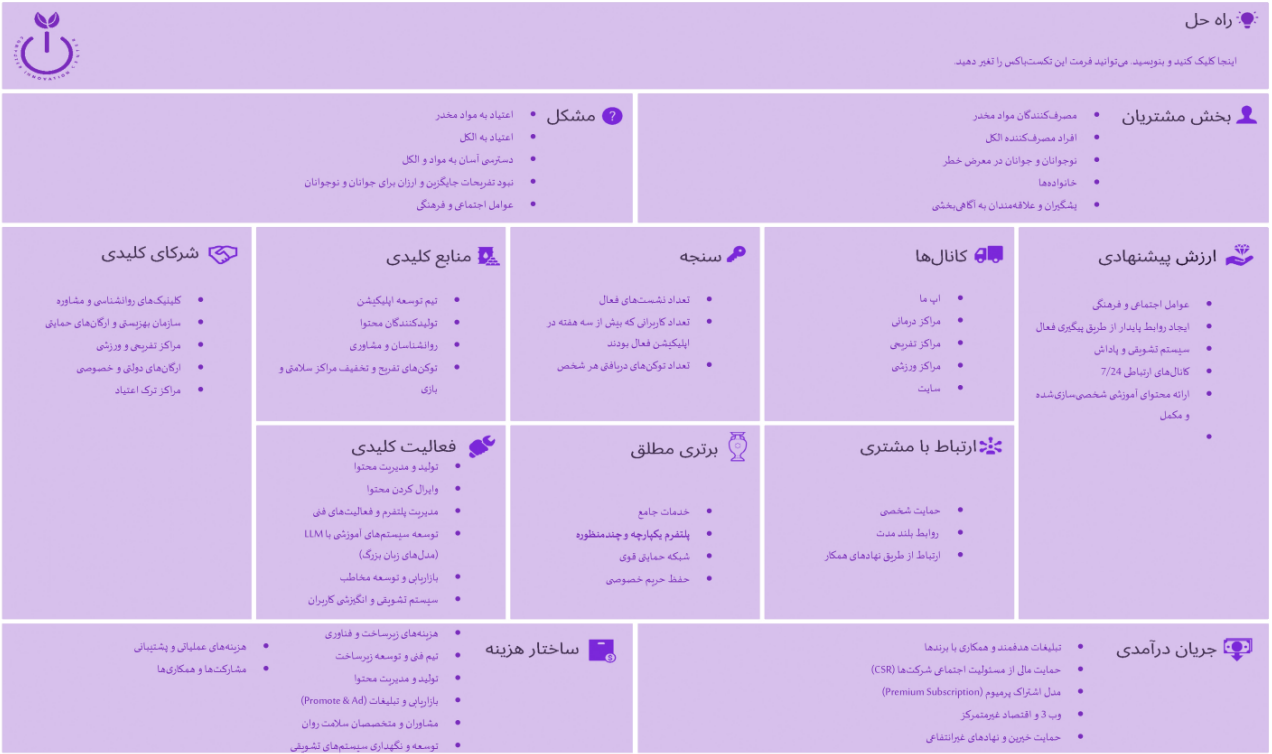
\includegraphics[scale=0.74, angle=90]{../images/canvas1}
\end{center}
\caption{مدل کسب و کار}
\label{fig:canvas}
\end{figure}

\subsection{چشم‌انداز، ماموریت‌ها و ارزش‌ها}
\subsubsection{چشم‌انداز‌ها}
ایجاد جهانی که در آن اعتیاد به مواد مخدر و الکل دیگر تهدیدی برای سلامت و کیفیت زندگی افراد نباشد و افراد جامعه به ابزارها، دانش و حمایت لازم برای پیشگیری و مقابله با این چالش دسترسی داشته باشند. هدف اصلی، ساختن جامعه‌ای است که در آن آگاهی، سلامت روانی و جسمی، و روابط اجتماعی پایدار و مثبت جایگزین اعتیاد شوند. این چشم‌انداز بر تغییر فرهنگ و ایجاد یک محیط امن و حمایتگر تأکید دارد که به رشد و پویایی فردی و اجتماعی کمک کند.

\subsubsection{ماموریت‌‌ها}
\begin{enumerate}
\item 
آگاهی‌بخشی عمومی

توسعه محتوای آموزشی متناسب با فرهنگ جامعه برای افزایش دانش مردم درباره عوارض و پیامدهای اعتیاد و اهمیت پیشگیری.  

\item 
تسهیل دسترسی به خدمات حمایتی

ایجاد بستری دیجیتال که ارتباط میان افراد در معرض خطر و مشاوران حرفه‌ای را تسهیل کرده و خدمات پیشگیرانه و درمانی را در دسترس همگان قرار دهد.  
\item 
ارتقای سلامت اجتماعی

همکاری با نهادهای مرتبط، کلینیک‌های تخصصی و سازمان‌های غیردولتی برای ایجاد هم‌افزایی و پیشبرد اهداف کاهش اعتیاد.  

\item 
نوآوری در راه‌حل‌ها

استفاده از فناوری‌های پیشرفته، مانند هوش مصنوعی و داده‌های کلان، برای شناسایی الگوهای رفتاری و ارائه راهکارهای شخصی‌سازی‌شده به کاربران.
\end{enumerate}

\subsubsection{ارزش‌ها}
\begin{enumerate}
\item 
صداقت و شفافیت

ارائه اطلاعات و خدمات با نهایت دقت و صحت، به‌گونه‌ای که اعتماد کاربران جلب شده و آنان به دریافت کمک تمایل پیدا کنند.  

\item 
حفظ کرامت انسانی

احترام به تمام افراد بدون توجه به پیشینه یا مشکلات آنان و ارائه راهکارهایی که حریم خصوصی و ارزش‌های انسانی را حفظ کنند.  

\item 
همکاری و مشارکت

ایجاد هم‌افزایی میان نهادها، خانواده‌ها و جوامع برای مقابله با اعتیاد و تقویت پیوندهای اجتماعی.  

\item 
تعهد اجتماعی

تلاش مداوم برای کاهش آسیب‌های ناشی از اعتیاد و حمایت از نسل‌های آینده برای رسیدن به جامعه‌ای سالم‌تر و آگاه‌تر.  

\item 
نوآوری و خلاقیت

بهره‌گیری از روش‌های جدید و ابزارهای دیجیتال برای ایجاد تأثیر بیشتر در آگاهی‌بخشی و پیشگیری.
\end{enumerate}
\subsection{برنامه بازاریابی}
\begin{enumerate}
\item 
تبلیغات در فضای مجازی 
 
\textbf{هدف}:
افزایش آگاهی عمومی و جذب کاربران به پلتفرم.  
\begin{itemize}
\item 
کمپین‌های شبکه‌های اجتماعی
\begin{itemize}
\item 
طراحی محتواهای جذاب و آموزشی شامل ویدیوهای کوتاه، اینفوگرافیک‌ها، و داستان‌های الهام‌بخش از افرادی که اعتیاد را ترک کرده‌اند.  

\item 
استفاده از پلتفرم‌هایی مانند اینستاگرام، تلگرام، توییتر و لینکدین برای به اشتراک‌گذاری محتوا.  

\item 
اجرای کمپین‌های تبلیغاتی هدفمند با استفاده از ابزارهای تبلیغاتی (\lr{Google Ads} و تبلیغات در شبکه‌های اجتماعی).  

\item 
دعوت از افراد تأثیرگذار (اینفلوئنسرها) برای حمایت از کمپین‌ها و تبلیغ ارزش‌های پلتفرم.  
\end{itemize}

\item 
استفاده از تبلیغات هدفمند
\begin{itemize}
\item 
تبلیغات مبتنی بر علاقه‌مندی کاربران در گروه‌های مختلف (مانند خانواده‌ها، جوانان و نوجوانان).  

\item 
ارائه کدهای تخفیف یا دسترسی رایگان به خدمات ویژه برای کاربران جدید.  
\end{itemize}
\item 
ایجاد محتوای ویروسی
\begin{itemize}
\item 
چالش‌های اجتماعی با هشتگ‌های مخصوص (مثلاً 
\textcolor{blue}{\#زندگی\_بدون\_اعتیاد}).  
\item 
داستان‌های کاربران موفق و محتوای انگیزشی برای جلب مشارکت بیشتر.  
\end{itemize}
\end{itemize}

\item 
تبلیغات شهری و مدارس 
 
\textbf{هدف}:
افزایش آگاهی عمومی به‌ویژه در میان نوجوانان و خانواده‌ها.  

\begin{itemize}
\item 
برگزاری کمپین‌های شهری
\begin{itemize}
\item 
نصب بیلبوردها و پوسترهای آموزشی در مناطق پرتردد شهری با پیام‌های انگیزشی و آموزشی.  
\item 
استفاده از ایستگاه‌های مترو، اتوبوس و پایانه‌های مسافربری برای تبلیغات کوتاه و هدفمند.  
\end{itemize}
\item 
فعالیت در مدارس
\begin{itemize}
\item 
برگزاری کارگاه‌ها و سخنرانی‌های آموزشی برای دانش‌آموزان، معلمان و والدین.  
\item 
توزیع بروشورها، کتابچه‌های آموزشی و پوسترهای جذاب در مدارس.  
\item 
معرفی اپلیکیشن یا خدمات از طریق مشاوران مدارس.  
\item 
راه‌اندازی مسابقات یا برنامه‌های مشارکتی در مدارس با موضوع مبارزه با اعتیاد.  
\end{itemize}
\item 
توزیع محتوای آگاهی‌بخش
\begin{itemize}
\item 
چاپ استیکرها و کارت‌های آموزشی با پیام‌های کوتاه و الهام‌بخش برای توزیع در مدارس و مکان‌های عمومی.  
\end{itemize}
\end{itemize}

\item 
استفاده از گیمیفیکیشن \lr{(Gamification)} 
 
\textbf{هدف}:
افزایش تعامل و مشارکت کاربران با استفاده از مکانیزم‌های بازی‌گونه.  
\begin{itemize}
\item 
سیستم پاداش
\begin{itemize}
\item 
ارائه امتیاز به کاربران برای تکمیل دوره‌های آموزشی در اپلیکیشن.  
\item 
ایجاد جدول امتیازات \lr{(Leaderboard)} برای تشویق رقابت سالم بین کاربران.  
\item 
جوایز مانند اشتراک رایگان، تخفیف خدمات یا هدایای نمادین برای کاربران فعال.  
\end{itemize}

\item 
بازی‌های آموزشی
\begin{itemize}
\item 
طراحی بازی‌هایی که به صورت غیرمستقیم مضرات اعتیاد را آموزش دهند (مانند شبیه‌سازی‌های زندگی سالم).  
\item 
استفاده از سناریوهایی که در آن‌ها کاربر تصمیم‌گیری‌های مهمی برای مقابله با چالش‌های مربوط به اعتیاد انجام می‌دهد.  
\end{itemize}

\item 
چالش‌های گروهی
\begin{itemize}
\item 
دعوت از کاربران به شرکت در چالش‌های گروهی مانند "30 روز بدون مواد مخدر`` و ارائه جوایز به گروه‌های برتر.  
\item 
طراحی فعالیت‌های اجتماعی که کاربران بتوانند امتیاز جمع کنند و اهداف مشخصی را با هم به پایان برسانند.  
\end{itemize}

\item 
تشویق معرفی به دیگران
\begin{itemize}
\item 
ارائه امتیاز به کاربران برای معرفی دوستان خود به پلتفرم.  
\item 
فعال‌سازی برنامه‌های همکاری کاربران برای تبلیغ پلتفرم در محیط‌های آموزشی و اجتماعی.  
\end{itemize}
\end{itemize}

\item 
برگزاری دورهمی‌های اجتماعی  

\textbf{هدف}:
تقویت ارتباطات اجتماعی و افزایش آگاهی از طریق فعالیت‌های گروهی.  

\begin{itemize}
\item 
دورهمی‌های آموزشی
\begin{itemize}
\item 
برگزاری رویدادهای حضوری در پارک‌ها، کتابخانه‌ها، یا مراکز فرهنگی با موضوعات مرتبط با آگاهی‌بخشی درباره اعتیاد.  
\item 
دعوت از متخصصان، روانشناسان و افراد موفق برای سخنرانی و تبادل تجربه.  
\item 
فراهم کردن فضای مشارکت جمعی برای بحث و گفت‌وگو درباره راهکارهای مقابله با اعتیاد.  
\end{itemize}

\item 
برنامه‌های تفریحی و فرهنگی
\begin{itemize}
\item 
سازمان‌دهی مسابقات ورزشی، نمایش فیلم‌های آموزشی و برنامه‌های هنری با پیام‌های مرتبط با زندگی سالم.  
\item 
ترکیب فعالیت‌های سرگرم‌کننده با آموزش غیرمستقیم درباره اعتیاد.  
\end{itemize}

\item 
جلسات حمایتی
\begin{itemize}
\item 
ایجاد گروه‌های حمایتی برای افرادی که به تازگی ترک کرده‌اند یا خانواده‌های آنان.  
\item 
استفاده از فضای دورهمی برای تقویت روحیه و ایجاد انگیزه در میان اعضای جامعه هدف.  
\end{itemize}
\end{itemize}

\item 
برنامه ریفرال \lr{(Referral Program)}  

\textbf{هدف}:
افزایش تعداد کاربران با استفاده از مشارکت کاربران فعلی.  
\begin{itemize}
\item 
سیستم پاداش برای معرفی دوستان
\begin{itemize}
\item 
ارائه امتیاز یا جوایز ویژه (مانند دسترسی به محتوای اختصاصی یا تخفیف در خدمات) برای کاربرانی که دوستان خود را به پلتفرم دعوت می‌کنند.  
\item 
طراحی کدهای ریفرال اختصاصی برای هر کاربر و رهگیری تعداد افرادی که از طریق آن کد ثبت‌نام کرده‌اند.  
\end{itemize}

\item 
تشویق کاربران به گسترش پیام آگاهی‌بخشی
\begin{itemize}
\item 
ارائه امتیاز برای اشتراک‌گذاری محتواهای پلتفرم در شبکه‌های اجتماعی.  
\item 
راه‌اندازی کمپین‌هایی با محوریت ریفرال، مانند "هر کاربری که 5 نفر را دعوت کند، یک جایزه ویژه دریافت می‌کند.``
\end{itemize}

\item 
برنامه‌های گروهی
\begin{itemize}
\item 
ایجاد تیم‌های دوستانه در پلتفرم و ارائه چالش‌های گروهی که افراد بیشتری را به مشارکت دعوت کند.
\item 
ارائه جوایز گروهی برای تیم‌هایی که تعداد بیشتری از اعضا را به جامعه اضافه کنند.
\end{itemize}
\end{itemize}
\end{enumerate}

\section{تحلیل‌های مالی}
\subsection{مقدمه}
پروژه اپلیکیشن مقابله با اعتیاد و پیشگیری از مصرف مواد مخدر و الکل، به عنوان یک ابزار نوین و فناورانه برای حل یکی از معضلات اجتماعی، نیازمند یک رویکرد مالی دقیق و هدفمند است.

در این تحلیل مالی، هدف اصلی شناسایی و مدیریت منابع مالی و هزینه‌های مربوط به مراحل مختلف توسعه و اجرای اپلیکیشن است. این تحلیل شامل بررسی هزینه‌های سرمایه‌ای برای توسعه نرم‌افزار، هزینه‌های عملیاتی مرتبط با پشتیبانی و به‌روزرسانی و همچنین پیش‌بینی منابع درآمدی برای اطمینان از پایداری مالی پروژه می‌باشد. علاوه بر این، سناریوهای مختلف فروش و استفاده از اپلیکیشن مورد بررسی قرار خواهد گرفت تا نقاط قوت و ضعف پروژه از منظر مالی شناسایی شود.

این تحلیل به تصمیم‌گیری هوشمندانه‌تر و اجرای بهینه‌تر پروژه کمک می‌کند و به شهرداری اصفهان این امکان را می‌دهد که منابع خود را در راستای رفع و پیشگیری از اعتیاد به صورت مؤثرتری به کار گیرد.

\subsection{قیمت‌گذاری و بیان دلایل}
حال در این قسمت به قیمت گذاری بر اساس بوم کسب و کار می‌پردازیم و برای تمامی موارد دلایل را توضیح می‌دهیم.

\subsubsection{مشتریان هدف و ارزش پیشنهادی}
\begin{itemize}
\item 
قیمت‌گذاری
\begin{itemize}
\item
مشتریان اصلی

نوجوانان، جوانان، خانواده‌ها، و افراد در معرض اعتیاد.

\item
استفاده رایگان با گزینه‌های پرداخت درون‌برنامه‌ای

کاربران می‌توانند به اکثر امکانات (مانند محتواهای آموزشی پایه و یادآورها) به‌صورت رایگان دسترسی داشته باشند، اما برای خدمات پیشرفته‌تر (مانند جلسات مشاوره اختصاصی، برنامه‌های سفارشی‌شده و چالش‌های ویژه) هزینه پرداخت کنند.

\item
اشتراک پرمیوم

اشتراک ماهانه
$100,000$
تومان یا سالانه
$1,000,000$
تومان برای دسترسی کامل به تمام امکانات.
\end{itemize}

\item 
دلایل
\begin{itemize}
\item
استفاده رایگان، کاربران بیشتری را جذب می‌کند و تأثیر اجتماعی پروژه را افزایش می‌دهد.

\item
گزینه‌های پرمیوم برای پشتیبانی مالی پایدار پروژه طراحی شده‌اند.

\item
خانواده‌ها و نوجوانان معمولاً بودجه محدودی دارند، بنابراین ارائه خدمات رایگان پایه، به جذب بیشتر کمک می‌کند.
\end{itemize}
\end{itemize}

\subsubsection{کانال‌ها \lr{(Channels)}}
\begin{itemize}
\item 
قیمت‌گذاری
\begin{itemize}
\item 
اپلیکیشن

هزینه توسعه و نگهداری اولیه در حدود
$200,000,000$
تومان (طراحی \lr{UI/UX}، توسعه، تست، و انتشار).

\item 
تبلیغات هدفمند

حدود
$50,000,000$
تومان برای تبلیغات در شبکه‌های اجتماعی و گوگل.

\item 
ارتباط با مراکز درمانی

تخصیص
$20,000,000$
تومان برای هماهنگی و انعقاد قرارداد با مراکز درمانی.
\end{itemize}

\item 
دلایل
\begin{itemize}
\item 
جذب کاربران از طریق اپلیکیشن اصلی کانال توزیع خدمات است.

\item 
تبلیغات دیجیتال باعث جذب سریع‌تر کاربران و ارتقای آگاهی عمومی می‌شود.

\item 
مراکز درمانی به عنوان همکار کلیدی، اعتماد کاربران را افزایش می‌دهند.
\end{itemize}
\end{itemize}

\subsubsection{فعالیت‌های کلیدی}
\begin{itemize}
\item 
قیمت‌گذاری
\begin{itemize}
\item
تولید محتوا

حدود
$50,000,000$
تومان برای تولید ویدئوهای آموزشی، مقالات، و چالش‌ها.

\item
برگزاری کمپین‌ها

حدود
$25,000,000$
تومان برای برگزاری کمپین‌های تفریحی، کمپینگ‌ها و فعالیت‌های گروهی.

\item
پشتیبانی و به‌روزرسانی اپلیکیشن

حدود
$32,000,000$
تومان در سال برای پشتیبانی نرم‌افزاری و رفع مشکلات.
\end{itemize}

\item 
دلایل
\begin{itemize}
\item
محتوای جذاب و متنوع به حفظ کاربران کمک می‌کند.

\item
کمپین‌ها باعث تعامل بیشتر و ایجاد حس تعلق در کاربران می‌شود.

\item
پشتیبانی مداوم، رضایت کاربران را تضمین می‌کند.
\end{itemize}
\end{itemize}

\subsubsection{منابع کلیدی}
  \begin{itemize}
\item 
قیمت‌گذاری
\begin{itemize}
\item 
سرورها و زیرساخت‌ها

حدود
$1,000,000$
تومان ماهانه برای اجاره سرور و سرویس‌های ابری.

\item 
تیم توسعه و مشاوره

هزینه تیم برنامه‌نویسان، طراحان، و روانشناسان حدود
$240,000,000$
تومان در سال.

\item 
مراکز همکار

تخصیص تخفیف‌های مالی یا مشوق‌ها به مراکز درمانی و تفریحی به میزان
$20,000,000$
تومان.
\end{itemize}

\item 
دلایل
\begin{itemize}
\item 
سرورها برای پشتیبانی از حجم بالای کاربران ضروری‌اند.

\item 
تخصص تیم توسعه و روانشناسان تضمین‌کننده کیفیت خدمات است.

\item 
همکاری با مراکز همکار ارزش افزوده بیشتری ایجاد می‌کند.
\end{itemize}
\end{itemize}

\subsubsection{ساختار هزینه‌ها}
\begin{itemize}
\item 
قیمت‌گذاری
\begin{itemize}
\item 
توسعه اولیه

حدود
$200,000,000$
تا
$320,000,000$
تومان برای طراحی و راه‌اندازی.

\item 
هزینه‌های تبلیغات

حدود
$80,000,000$
تومان برای تبلیغات و معرفی پروژه.

\item 
هزینه‌های عملیاتی

حدود
$100,000,000$
تومان سالانه برای نگهداری، به‌روزرسانی، و خدمات پشتیبانی.
\end{itemize}

\item 
دلایل
\begin{itemize}
\item
هزینه‌های توسعه و تبلیغات برای شروع موفق پروژه ضروری است.
\item 
هزینه‌های عملیاتی برای تضمین عملکرد پایدار اپلیکیشن مورد نیاز است.
\end{itemize}
\end{itemize}

\subsubsection{جریان‌های درآمدی}
\begin{itemize}
\item 
قیمت‌گذاری
\begin{itemize}
\item 
پرداخت درون‌برنامه‌ای

قیمت‌گذاری خدمات از
$20,000$
تومان تا
$500,000$
تومان (بسته به نوع خدمات).

\item 
اشتراک پرمیوم
$100,000$
تومان ماهانه یا
$1,000,000$
تومان سالانه.

\item 
تبلیغات هدفمند

درآمد سالانه
$150,000,000$
تومان از تبلیغات مرتبط.

\item 
همکاری با شرکت‌ها و سازمان‌ها \lr{(CSR)}

دریافت حمایت مالی
$500,000,000$
تومان از شرکت‌های مسئولیت‌پذیر اجتماعی.
\end{itemize}

\item 
دلایل
\begin{itemize}
\item 
قیمت‌گذاری رقابتی و مقرون‌به‌صرفه برای جذب کاربران بیشتر.
\item 
اشتراک پرمیوم و تبلیغات به تأمین مالی پایدار پروژه کمک می‌کند.
\item 
همکاری با شرکت‌ها علاوه بر منابع مالی، اعتبار پروژه را افزایش می‌دهد.
\end{itemize}
\end{itemize}

\subsection{سناریوهای فروش و پیش‌بینی‌ها \lr{(Sales Scenarios and Projections)}}
\subsubsection{سناریو فروش پایه \lr{(Base Scenario)}}
در این سناریو، تمرکز بر جذب کاربران رایگان است که به آموزش‌های عمومی، یادآورها، و بازی‌های ساده دسترسی دارند. هدف این است که از طریق استفاده گسترده کاربران و ایجاد آگاهی، نرخ جذب \lr{(Acquisition Rate)} به بالاترین حد ممکن برسد.

\begin{itemize}
\item 
خدمات رایگان

شامل محتواهای آموزشی پایه، چالش‌های ابتدایی، و ابزارهای پیگیری عمومی.
\item 
درآمدزایی

این سناریو بر درآمدزایی غیرمستقیم از طریق تبلیغات هدفمند و حمایت‌های دولتی یا سازمان‌های مسئولیت‌پذیر اجتماعی \lr{(CSR)} تکیه دارد.
\end{itemize}

پیش‌بینی‌ها
\begin{itemize}
\item 
تعداد کاربران فعال ماهانه

$50,000$
نفر در سال اول.
\item 
درآمد تبلیغاتی سالانه

$150,000,000$
تومان از تبلیغات هدفمند.
\item 
حمایت‌های دولتی و \lr{CRS} سالانه

$500,000,000$
تومان.
\end{itemize}


\subsubsection{سناریوی درآمدزایی از اشتراک پرمیوم \lr{(Premium Subscription Scenario)}}
در این سناریو، خدمات پیشرفته‌ای به کاربران ارائه می‌شود که شامل برنامه‌های شخصی‌سازی‌شده، مشاوره‌های تخصصی روانشناسی، و دسترسی کامل به تمام ویژگی‌های اپلیکیشن است. کاربران علاقه‌مند به سلامت روان و ترک اعتیاد می‌توانند با پرداخت اشتراک، از این امکانات استفاده کنند.
\begin{itemize}
\item
اشتراک ماهانه/سالانه

هزینه
$100,000$
تومان ماهانه یا
$1,000,000$
تومان سالانه برای هر کاربر.

\item
ارائه تخفیف گروهی

تخفیف‌های جذاب برای خانواده‌ها یا مراکز درمانی که چندین اشتراک خریداری می‌کنند.
\end{itemize}
پیش‌بینی‌ها

\begin{itemize}
\item 
تعداد کاربران پرمیوم

500 نفر در سال اول.
\item 
درآمد سالانه از اشتراک

$500,000,000$
تومان.
\item 
نرخ رشد کاربران پرمیوم

20\% افزایش سالانه.
\end{itemize}

\subsubsection{سناریوی مبتنی بر مشارکت اجتماعی \lr{(Community Engagement Scenario)}}
این سناریو بر تقویت مشارکت اجتماعی کاربران و ارائه خدمات ارزشمند از طریق بازی‌سازی \lr{(Gamification)} و سیستم‌های پاداش متمرکز است. در این حالت، کاربران برای انجام فعالیت‌های سالم و مشارکت در چالش‌های گروهی، توکن یا امتیاز دریافت می‌کنند که می‌توانند از آن‌ها برای تخفیف خدمات یا استفاده از امکانات تفریحی و ورزشی بهره ببرند.

\begin{itemize}
\item
مدل درآمدی

فروش توکن و همکاری با مراکز همکار (تفریحی، درمانی، و ورزشی).

\item
مکانیزم تشویق

کاربران با خرید توکن بیشتر، امکانات ویژه‌ای دریافت می‌کنند.
\end{itemize}
پیش‌بینی‌ها

\begin{itemize}
\item 
 فروش 5000 توکن به قیمت متوسط

$10,000$
تومان در سال اول.
\item 
درآمد از فروش توکن

$50,000,000$
تومان در سال.
\item 
مشارکت مراکز همکار

$500,000,000$
تومان در قالب تخفیف و همکاری.
\end{itemize}


\subsubsection{سناریوی فروش خدمات مشاوره \lr{(Counseling Services Scenario)}}
در این سناریو، خدمات مشاوره‌ای تخصصی از طریق جلسات آنلاین یا حضوری به کاربران ارائه می‌شود. این خدمات توسط تیمی از روانشناسان و مشاوران حرفه‌ای انجام می‌شود و هزینه هر جلسه بر اساس نوع خدمات متفاوت خواهد بود.
\begin{itemize}
\item
جلسات آنلاین

هزینه هر جلسه
$100,000$
تا
$300,000$
تومان.

\item
بسته‌های مشاوره

بسته‌های تخفیفی شامل چندین جلسه مشاوره برای جذب بیشتر مشتریان.
\end{itemize}

پیش‌بینی‌ها:
\begin{itemize}
\item
تعداد جلسات مشاوره

2500 جلسه در سال اول.

\item
درآمد از مشاوره

$500,000,000$
تومان در سال اول.

\item
رضایت کاربران 

پیش‌بینی نرخ رضایت 90\% برای افزایش مشتریان وفادار.
\end{itemize}


\subsubsection{سناریوی اشتراک سازمانی \lr{(Corporate Subscription Scenario)}}
این سناریو بر همکاری با شرکت‌ها، مدارس، و سازمان‌های مختلف برای ارائه خدمات گروهی و اشتراکی تمرکز دارد. شرکت‌ها و سازمان‌ها می‌توانند اشتراک سازمانی خریداری کرده و به کارمندان یا اعضای خود خدمات ویژه ارائه دهند.

\begin{itemize}
\item
مدل اشتراک

پلن‌های اشتراک سالانه برای سازمان‌ها به ازای هر کاربر
$1,000,000$
تومان.

\item
همکاری با مدارس و نهادهای آموزشی

ارائه خدمات ویژه به دانش‌آموزان و معلمان برای پیشگیری از اعتیاد.
\end{itemize}

پیش‌بینی‌ها

\begin{itemize}
\item
تعداد کاربران سازمانی

200 کاربر در سال اول.

\item
درآمد سالانه
$200,000,000$
تومان.

\item
رشد سالانه

15\% افزایش تعداد کاربران سازمانی.
\end{itemize}

\subsubsection{پیش‌بینی کلی پروژه \lr{(Overall Projections)}}
با ترکیب سناریوهای فوق، پیش‌بینی می‌شود که پروژه در سال اول به اهداف زیر دست یابد

\begin{itemize}
\item 
تعداد کاربران رایگان

$50,000$
نفر.

\item 
تعداد کاربران پرمیوم

500 نفر.

\item 
درآمد سالانه از کاربران رایگان (تبلیغات و حمایت‌ها) 

$150,000,000$
تومان از تبلیغات هدفمند +
$500,000,000$
تومان از حمایت‌های دولتی پس
$\text{\lr{CRS}} = 650,000,000$
تومان

\item 
درآمد سالانه از اشتراک پرمیوم

$500,000,000$
تومان

\item 
درآمد سالانه از فروش توکن‌ها

$50,000,000$
تومان

\item 
درآمد سالانه از مشاوره

$500,000,000$
تومان

\item 
درآمد سالانه از اشتراک سازمانی

$200,000,000$
تومان

\item 
کل درآمد سال اول

$1,900,000,000$
تومان
\end{itemize}

در پایان سال دوم، هزینه‌های اولیه پروژه پوشش داده شده و سوددهی آغاز می‌شود.

نوآوری‌ها و جذابیت‌ها در سناریوهای فروش
\begin{enumerate}
\item 
سیستم گیمیفیکیشن و پاداش

کاربران از طریق بازی‌های تعاملی و چالش‌های گروهی جذب می‌شوند و انگیزه‌ای برای استفاده مداوم از اپلیکیشن پیدا می‌کنند.

\item
ارائه خدمات شخصی‌سازی‌شده

از هوش مصنوعی برای ارائه محتوا و پیشنهادات متناسب با نیازهای هر کاربر استفاده می‌شود.

\item 
حمایت اجتماعی

همکاری با سازمان‌های دولتی و غیردولتی برای تأمین منابع مالی و ارتقای آگاهی عمومی.

\item 
پایداری مالی

تنوع در مدل‌های درآمدی (پرداخت درون‌برنامه‌ای، اشتراک، تبلیغات، و همکاری با مراکز) پایداری مالی پروژه را تضمین می‌کند.
\end{enumerate}

\subsection{تحلیل‌ دقیق هزینه‌ها}
\begin{table}[H]
\begin{center}
\caption{تحلیل دقیق هزینه‌ها}
\begin{tabular}{p{0.35\textwidth}|p{0.15\textwidth}|p{0.35\textwidth}}
توضیحات &
\raggedleft
هزینه (تومان) &
جزئیات \\
\hline
\hline
توسعه امکانات خاص (مثل مشاوره آنلاین) &
\raggedright
$50,000,000$ &
اضافه کردن ویژگی‌های منحصر به فرد
\\ \hline

تست عملکرد \lr{(Performance test)}
&
\raggedright
$5,000,000$
&
تست کارایی اپلیکیشن تحت فشار و بار سنگین
\\ \hline
رفع باگ‌ها و بهینه‌سازی
&
\raggedright
$25,000,000$
&
رفع خطا‌‌ها و بهبود عملکرد اپلیکیشن
\\ \hline

کدنویسی و توسعه‌ی بک‌اند
&
\raggedright
$20,000,000$
&
برنامه‌‌‌نویسی سرور و مدیریت داده‌‌ها
\\ \hline
کدنویسی و توسعه‌ی فرانت‌اند
&
\raggedright
$15,000,000$
&
برنامه‌نویسی رابط کاربری برای کاربر نهایی
\\ \hline
پیاده‌سازی گیمیفیکیشن
&
\raggedright
$5,000,000$
&
اضافه کردن المان‌های تعاملی و جذاب
\\ \hline
پیاده‌سازی هوش مصنوعی
&
\raggedright
$10,000,000$
&
توسعه‌ی الگوریتم‌های هوشمند
\\ \hline
طراحی تجربه‌ی کاربری
&
\raggedright
$7,000,000$
&
طراحی تعاملات کاربر با اپلیکیشن
\\ \hline
\end{tabular}

\caption{هزینه‌های خدماتی}
\begin{tabular}
{p{0.35\textwidth}|p{0.15\textwidth}|p{0.35\textwidth}}
توضیحات &
هزینه (تومان) &
جزئیات \\
\hline
\hline
حقوق تیم پشتیبانی (۲ نفر)
&
\raggedright
$15,000,000 \times \text{12 ماه} = 180,000,000$
&
هزینه حقوق پشتیبانی به صورت ماهانه
\\ \hline
سیستم مدیریت تیکت‌ها
&
\raggedright
$5,000,000$
&
هزینه‌ی راه‌اندازی و نگهداری مدیریت تیکت‌ها
\\ \hline
راه‌اندازی بخش پرسش‌های متداول
&
\raggedright
$12,000,000$
&
هزینه‌ی طراحی و پیاده‌سازی بخش 
\lr{FAQ}
\\ \hline
تماس‌های پشتیبانی
&
\raggedright
$3,000,000$
&
هزینه‌های مربوط به تماس‌های پشتیبانی و تلفن
\\ \hline
نظرسنجی و تحلیل بازخورد کاربران
&
\raggedright
$8,000,000$
&
هزینه‌ی نظرسنجی از کاربران و تحلیل داده‌های بازخورد
\\ \hline
آموزش مداوم تیم پشتبانی
&
\raggedright
$4,000,000$
&
هزینه‌ی دوره‌های آموزشی برای ارتقا مهارت‌های تیم پشتیبانی
\\ \hline

پشتیبانی ۲۴/۷ از طریق ایمیل
& 
\raggedright
$5,000,000$
& 
هزینه‌ی مربوط به پشتیبانی ایمیلی برای کاربران در تمام ساعات شبانه‌روز
\\ \hline
\end{tabular}

\caption{تحلیل هزینه‌های تبلیغات}
\begin{tabular}{p{0.35\textwidth}|p{0.15\textwidth}|p{
0.35\textwidth}}
توضیحات &
هزینه سالانه (ت) &
جزئیات \\
\hline
\hline
تبلیغات شبکه‌های اجتماعی
&
\raggedright
$30,000,000$
&
هزینه‌ی تبلیغات در پلتفرم‌های اجتماعی مانند اینستاگرام و تلگرام
\\ \hline

تبلیغات 
\lr{Google Ads}
&
\raggedright
$40,000,000$
&
تبلیغات در گوگل برای جذب کاربران هدف
\\ \hline

طراحی ویدیو‌های تبلیغاتی
&
\raggedright
$15,000,000$
&
هزینه‌ی طراحی و تولید ویدیو‌های تبلیغاتی
\\ \hline

همکاری با اینفلوئنسر‌ها
&
\raggedright
$30,000,000$
&
همکاری با افراد تاثیرگذار در شبکه‌های اجتماعی برای تبلیغات
\\ \hline

چاپ بروشور و کاتالوگ
&
\raggedright
$10,000,000$
&
هزینه‌ی طراحی و چاپ بروشورها و کاتالوگ‌های تبلیغاتی
\\ \hline

برگزاری رویداد‌ها و نمایشگاه‌ها
&
\raggedright
$20,000,000$
&
هزینه‌های مربوط به حضور در نمایشگاه‌ها و برگزاری رویداد‌های تبلیغاتی
\\ \hline

ارائه تخفیف‌های ویژه تبلیغاتی
&
\raggedright
$20,000,000$
&
هزینه‌های تخفیف‌های ویژه
\\ \hline

\end{tabular}
\end{center}
\end{table}

\begin{table}[H]
\begin{center}
\caption{هزینه‌های زیرساخت و فناوری}
\begin{tabular}{p{0.35\textwidth}|p{0.15\textwidth}|p{
0.35\textwidth}}
توضیحات &
هزینه سالانه (ت) &
جزئیات \\
\hline
\hline

اجازه سرور و سرویس‌های ابری
&
\raggedright
$12 \times 2,000,000 = 24,000,000$
&
هزینه اجاره سرور و استفاده از سرویس‌های ابری برای ذخیره‌سازی داده‌ها
\\ \hline

هزینه‌ی پایگاه داده
&
\raggedright
$10,000,000$
&
هزینه نگهداری و مدیریت پایگاه داده برای اپلیکیشن
\\ \hline

تمدید دامنه و هاست
&
\raggedright
$24,000,000 \times \text{\%x}$
&
هزینه تمدید دامنه و سرویس‌های هاست برای نگهداری وب‌سایت
\\ \hline

لایسنس نرم‌افزارها
&
\centering
-
&
هزینه خرید و تمدید لایسنس نرم‌افزارهای ضروری
\\ \hline

بهینه‌سازی زیرساخت
&
\centering
-
&
هزینه بهینه‌سازی زیرساخت‌ها برای عملکرد بهتر اپلیکیشن
\\ \hline
\end{tabular}
\end{center}
\end{table}

به علت ریموت بودن ماهیت کسب و کار هزینه‌های مربوط به محل کار آورده نشده‌اند.
\subsection{تحلیل دقیق نقطه‌‌ی سر به سر}
 ابتدا باید داده‌های موجود را بررسی کرده و هزینه‌ها، درآمدها و قیمت‌گذاری را در نظر بگیریم. در اینجا، بر اساس داده‌های تحلیل مالی، به محاسبه‌ی نقطه سر به سر پرداخته و جزئیات مربوط به آن را مشاهده خواهید کرد.

\begin{enumerate}
\item 
هزینه‌های ثابت 
\lr{Fixes Costs}

هزینه‌های ثابت شامل تمامی هزینه‌هایی هستند که به‌طور مستقل از حجم فروش باقی می‌مانند.
\begin{itemize}
\item 
هزینه اجاره دفتر کار

$120,000,000$
تومان سالانه

\item 
هزینه‌های مربوط به زیرساخت‌ها و فناوری

$2,000,000$
تومان سالانه (هزینه اجاره سرور و سرویس‌های ابری)

\item 
هزینه‌های پشتیبانی

$180,000,000$
تومان سالانه (حقوق تیم پشتیبانی)

\item 
هزینه‌های تبلیغات و معرفی پروژه 

$80,000,000$
تومان (تبلیغات در شبکه‌های اجتماعی، گوگل و همکاری با اینفلوئنسرها)

\item 
هزینه‌های مرتبط با طراحی، توسعه، و بهینه‌سازی

شامل
$200,000,000$
تا
$320,000,000$
تومان برای توسعه نرم‌افزار و ویژگی‌های جدید

\item 
هزینه‌های عمومی اداره دفتر و تجهیزات

$55,000,000$
تومان (شامل هزینه خرید تجهیزات اداری و لوازم مصرفی)
\end{itemize}
مجموع هزینه‌های ثابت سالانه:
\begin{equation*}
120,000,000 + 24,000,000 + 180,000,000 + 80,000,000 + 200,000,000 = 604,000,000
\end{equation*}

\item 
 هزینه‌های متغیر \lr{(Variable Costs)}

هزینه‌های متغیر شامل هزینه‌هایی هستند که بسته به حجم فروش یا استفاده از خدمات تغییر می‌کنند. در پروژه‌ی ما، هزینه‌های متغیر به ازای هر کاربر یا هر استفاده از خدمات مختلف تعیین می‌شوند.

\begin{itemize}
\item 
هزینه تولید محتوا

$50,000,000$
تومان سالانه

\item 
هزینه‌های خدمات مشاوره و پشتیبانی

$5,000,000$
تومان برای پشتیبانی ۲۴/۷ و نظرسنجی از کاربران

\item 
هزینه‌های فروش و تبلیغات

$40,000,000$
تومان سالانه برای تبلیغات هدفمند
\end{itemize}

مجموع هزینه‌های متغیر سالانه:
\begin{equation*}
50,000,000 + 5,000,000 + 40,000,000 = 95,000,000
\end{equation*}

\item 
قیمت فروش واحد \lr{(Price per Unit)}

در پروژه‌ی ما، قیمت‌گذاری به صورت "پرداخت درون‌برنامه‌ای`` و "اشتراک پرمیوم`` است. بر اساس سناریوهای ارائه‌شده، ما می‌توانیم از این دو مدل درآمدی استفاده کنید.

\begin{itemize}
\item 
اشتراک پرمیوم

$100,000$
تومان ماهانه یا
$1,000,000$
تومان سالانه

\item 
پرداخت درون‌برنامه‌ای

از
$20,000$
تا
$500,000$
تومان برای هر خدمت خاص
\end{itemize}

برای محاسبه نقطه سر به سر، ما به عنوان یک فرضیه، از اشتراک پرمیوم سالانه استفاده می‌کنیم که
$1,000,000$
تومان است.

\item 
محاسبه نقطه سر به سر \lr{(Break-even Point)}

برای محاسبه نقطه سر به سر، از فرمول زیر استفاده می‌کنیم
\begin{equation}
\text{نقطه‌ی سر به سر} =
\frac{\text{هزینه‌ی ثابت کل}}{\text{قیمت فروش واحد} - \text{هزینه‌ی متغیر هر واحد}}
\end{equation}

در اینجا
\begin{itemize}
\item 
هزینه ثابت کل = $604,000,000$ تومان

\item 
قیمت فروش واحد = $1,000,000$ تومان

\item 
هزینه متغیر هر واحد = $95,000,000$ تومان (مجموع هزینه‌های متغیر)
\end{itemize}

محاسبه نقطه سر به سر:
\begin{equation}
\frac{604,000,000}{1,000,000 - \frac{95,000,000}{50,000}} \approx 604
\end{equation}

بنابراین، ما باید 604 اشتراک پرمیوم بفروشیم تا تمام هزینه‌های ثابت و متغیر پروژه پوشش داده شود و به نقطه سر به سر برسیم.
\end{enumerate}

نکات
\begin{itemize}
\item 
هزینه‌های ثابت: این هزینه‌ها برای شروع و راه‌اندازی پروژه ضروری هستند و باید پیش از فروش هر محصول یا خدمت پرداخت شوند.

\item 
هزینه‌های متغیر: این هزینه‌ها با افزایش تعداد کاربران یا استفاده از خدمات رشد خواهند کرد. از آنجا که این هزینه‌ها به ازای هر کاربر تغییر می‌کنند، برای رسیدن به نقطه سر به سر باید تعداد خاصی از کاربران یا اشتراک‌های پرمیوم فروخته شود.

\item 
نقطه سر به سر: در این محاسبه، شما به این نتیجه می‌رسید که برای پوشش تمامی هزینه‌ها، باید 604 اشتراک پرمیوم بفروشید. اگر بتوانید از این تعداد بیشتر فروش کنید، کسب‌وکار به سودآوری خواهد رسید.
\end{itemize}
این تحلیل نقطه سر به سر به ما کمک می‌کند که درک بهتری از حجم فروش مورد نیاز برای پوشش هزینه‌ها داشته باشیم. علاوه بر این، می‌توانیم استراتژی‌های فروش و تبلیغات خود را به گونه‌ای تنظیم کنیم که بتوانیم به این نقطه برسیم و از آن عبور کنیم.


\subsection{تحلیل سرمایه‌ی مورد نیاز}
در این بخش، هدف این است که محاسبه کنیم برای راه‌اندازی و شروع پروژه اپلیکیشن مقابله با اعتیاد، به چه میزان سرمایه اولیه نیاز است. این سرمایه برای هزینه‌های توسعه، تبلیغات، زیرساخت‌ها، و پشتیبانی پروژه ضروری است

\subsubsection{هزینه‌های سرمایه‌ای \lr{(Capital Costs)}}
\begin{enumerate}
\item[\thesubsubsection.1]
این هزینه‌ها مربوط به تمامی مخارجی هستند که برای راه‌اندازی پروژه نیاز است و معمولاً در ابتدا پرداخت می‌شوند. بر اساس تحلیل‌های قبلی، این هزینه‌ها شامل موارد زیر هستند
\begin{itemize}
\item 
توسعه اپلیکیشن و نرم‌افزار

هزینه طراحی و توسعه نرم‌افزار بین
$200,000,000$
تا
$320,000,000$
تومان است.

\item 
تجهیزات و زیرساخت‌ها

اجاره سرورها و سرویس‌های ابری به‌طور ماهانه $1,000,000$ تومان است.

\item 
تبلیغات دیجیتال

هزینه تبلیغات در شبکه‌های اجتماعی و گوگل حدود $50,000,000$ تومان است.

\item 
ارتباطات و همکاری با مراکز درمانی

برای همکاری با مراکز درمانی و سایر شرکا
$200,000,000$
تومان تخصیص داده شده است.

\item 
تولید محتوا

هزینه تولید محتوا (ویدئو، مقالات آموزشی، چالش‌ها) حدود
$50,000,000$
تومان است.
\end{itemize}
مجموع هزینه‌های سرمایه‌ای

$200,000,000+50,000,000+320,000,000+50,000,000+20,000,000=640,000,000$

\item[\thesubsubsection.2]
هزینه‌های عملیاتی \lr{(Operational Costs)}

هزینه‌های عملیاتی مربوط به هزینه‌هایی است که برای نگهداری، به‌روزرسانی و پشتیبانی سالانه پروژه ضروری هستند.
\begin{itemize}
\item 
پشتیبانی و نگهداری نرم‌افزار

هزینه سالانه پشتیبانی و رفع مشکلات حدود $32,000,000$ تومان است.

\item 
حقوق تیم پشتیبانی

هزینه حقوق تیم پشتیبانی (2 نفر) به‌طور ماهانه 15,000,000 تومان است که برای 12 ماه به 180,000,000 تومان می‌رسد.

\item 
هزینه سیستم‌های پشتیبانی (تیکت‌ها، پشتیبانی تلفنی و ایمیلی)

هزینه‌های مربوط به سیستم مدیریت تیکت‌ها، پشتیبانی 24/7 از طریق تلفن و ایمیل مجموعاً به 15,000,000 تومان در سال می‌رسد.

\item 
تبلیغات و کمپین‌های بازاریابی

هزینه سالانه تبلیغات و کمپین‌های دیجیتال حدود 80,000,000 تومان است.
\end{itemize}
\end{enumerate}

\subsubsection{نحوه هزینه‌کرد سرمایه \lr{(Capital Allocation)}}
در این بخش، باید مشخص کنیم که چگونه این سرمایه در پروژه هزینه خواهد شد. سرمایه اولیه و هزینه‌های عملیاتی باید به بخش‌های مختلف پروژه تخصیص یابد تا در مراحل مختلف توسعه، اجرای اپلیکیشن و پشتیبانی از آن، به‌طور مؤثر استفاده شود.

\begin{enumerate}
\item 
تخصیص سرمایه اولیه

\begin{itemize}
\item 
توسعه نرم‌افزار

بخش عمده سرمایه اولیه، یعنی حدود
$200,000,000$
تا
$320,000,000$
تومان برای طراحی و توسعه نرم‌افزار هزینه خواهد شد. این هزینه شامل طراحی رابط کاربری، برنامه‌نویسی سرور و نرم‌افزارهای مورد نیاز برای اپلیکیشن است.

\item 
زیرساخت‌ها

بخش دیگر هزینه اولیه، یعنی حدود 
$1,000,000$
تومان ماهانه برای اجاره سرورها و سرویس‌های ابری است که در مجموع برای یک سال حدود
$12,000,000$
تومان می‌شود.

\item 
تبلیغات و بازاریابی

هزینه اولیه تبلیغات برای جذب کاربران جدید حدود
$50,000,000 $
تومان است.

\item 
مراکز درمانی و همکاری‌های استراتژیک

هزینه‌هایی برای ایجاد روابط و همکاری با مراکز درمانی و سایر نهادهای همکار، به میزان 
$20,000,000$
تومان تخصیص داده شده است.
\end{itemize}

\item 
تخصیص هزینه‌های عملیاتی

\begin{itemize}
\item 
پشتیبانی نرم‌افزاری

برای پشتیبانی سالانه نرم‌افزار،
$32,000,000$
تومان هزینه خواهد شد که برای رفع مشکلات و به‌روزرسانی‌های اپلیکیشن صرف می‌شود.

\item 
هزینه‌های نیروی انسانی

برای تیم پشتیبانی (2 نفر) حقوق ماهانه
$15,000,000$
تومان خواهد بود که برای 12 ماه معادل
$180,000,000$
تومان خواهد شد.

\item 
تبلیغات و ارتقای پروژه

بودجه تبلیغات برای سالانه 
$80,000,000$
تومان است که شامل هزینه‌های تبلیغاتی در شبکه‌های اجتماعی، گوگل و همکاری با اینفلوئنسرها می‌شود.

\item 
مدیریت سیستم پشتیبانی و خدمات مشتری

هزینه‌های مرتبط با سیستم مدیریت تیکت‌ها، پشتیبانی 24/7 و نظرسنجی از کاربران حدود
$15,000,000$
تومان است.
\end{itemize}
\end{enumerate}

نتیجه‌گیری تحلیل سرمایه مورد نیاز و نحوه هزینه‌کرد آن

سرمایه اولیه برای راه‌اندازی پروژه حدود
$640,000,000$
تومان خواهد بود که شامل هزینه‌های توسعه نرم‌افزار، زیرساخت‌ها، تبلیغات و هماهنگی با مراکز درمانی است. این سرمایه برای راه‌اندازی و شروع پروژه ضروری است.
برای هزینه‌های سالانه، مبلغ
$307,000,000$
تومان برای پشتیبانی و به‌روزرسانی نرم‌افزار، تبلیغات، و حقوق تیم پشتیبانی تخصیص داده خواهد شد.
سرمایه‌گذاری و هزینه‌کرد این مبلغ به‌طور مؤثر می‌تواند موفقیت پروژه را در رسیدن به اهدافش تضمین کند و از پایدار ماندن پروژه در درازمدت حمایت کند.
\section{تحلیل عوامل محیطی}
\begin{enumerate}
\item 
نیروهای بازار \lr{(Market Forces)}

\begin{itemize}
\item 
نیازها و خواسته‌های مشتریان

بوم، مشتریان هدف را به وضوح مشخص می‌کند: افرادی که با اعتیاد (مواد مخدر و الکل) دست و پنجه نرم می‌کنند، افراد در حال بهبودی و افرادی که به دنبال پیشگیری از اعتیاد هستند. این بوم به نیاز به منابع قابل دسترسی و مقرون به صرفه، از جمله محتوای آموزشی، حمایت جامعه و راهنمایی شخصی پاسخ می‌دهد.

\item
بخش‌های بازار

این بوم، بخش گسترده‌ای از مشتریان را هدف قرار می‌دهد، از جمله افراد درگیر با انواع مختلف اعتیاد، خانواده‌های آنها و افرادی که به پیشگیری از اعتیاد علاقه دارند. این بوم نیازها و ترجیحات متنوع در این بخش را تشخیص می‌دهد.

\item
هزینه‌های تعویض

این پلتفرم با ایجاد محتوای شخصی‌سازی شده، مشارکت جامعه و پشتیبانی بلندمدت، تلاش می‌کند تا روابط قوی با کاربران ایجاد کند. این می‌تواند هزینه‌های تعویض را افزایش دهد و برای کاربران دشوارتر شود تا راه حل‌های جایگزین با سطح مشابهی از تعامل و پشتیبانی پیدا کنند.
\end{itemize}

\item 
روندهای کلیدی \lr{(Key Trends)}

\begin{itemize}
\item
روندهای فناوری

این کسب‌وکار به طور گسترده از فناوری استفاده می‌کند، از جمله یک برنامه تلفن همراه، پلتفرم‌های رسانه‌های اجتماعی و احتمالاً مدل‌های زبانی مبتنی بر هوش مصنوعی برای ایجاد محتوا و پشتیبانی شخصی‌سازی شده. این امر با روند رو به رشد سلامت دیجیتال و پزشکی از راه دور همسو است.

\item
روندهای اجتماعی و فرهنگی

این بوم، افزایش آگاهی و نگرانی در مورد اعتیاد در جامعه را مورد توجه قرار می‌دهد. این پلتفرم از تقاضای رو به رشد برای منابع سلامت روان قابل دسترسی و مقرون به صرفه و استفاده فزاینده از فناوری برای سلامت و تندرستی بهره می‌برد.
\end{itemize}

\item 
نیروهای صنعت \lr{(Industry Forces)}

\begin{itemize}
\item
رقبا

بوم، احتمالاً با مراکز توانبخشی سنتی، گروه‌های حمایتی اعتیاد و سایر پلتفرم‌های سلامت دیجیتال که به سلامت روان و اعتیاد می‌پردازند، رقابت می‌کند. این بوم باید با ارائه ترکیبی منحصر به فرد از محتوای آموزشی، حمایت جامعه و راهنمایی شخصی، خود را متمایز کند.

\item
ورودهای جدید

بازار سلامت دیجیتال و حمایت از اعتیاد پویا است و ممکن است شرکت‌های جدیدی را جذب کند. بوم باید تهدیدات بالقوه ناشی از رقبا جدید را در نظر گرفته و استراتژی‌هایی برای حفظ مزیت رقابتی خود توسعه دهد.

\item
محصولات و خدمات جایگزین

محصولات و خدمات جایگزین بالقوه شامل مشاوره سنتی، گروه‌های حمایتی و منابع خودیاری هستند. این پلتفرم باید با ارائه جایگزینی قابل دسترسی‌تر، مقرون به صرفه‌تر و جذاب‌تر، ارزش پیشنهادی خود را نشان دهد.
\end{itemize}

\item
نیروهای کلان اقتصادی \lr{(Macroeconomic Forces)}

\begin{itemize}
\item
شرایط بازار جهانی

مدل کسب‌وکار به شرایط کلی اقتصادی حساس است. رکود اقتصادی ممکن است شیوع اعتیاد را افزایش دهد و بر مقرون به صرفه بودن خدمات مراقبت‌های بهداشتی، از جمله خدمات ارائه شده توسط این پلتفرم، تأثیر بگذارد.

\item
بازارهای سرمایه

دسترسی به بودجه برای توسعه و مقیاس‌بندی پلتفرم بسیار مهم است. بوم باید گزینه‌های تامین مالی، مانند سرمایه خطرپذیر، کمک‌های مالی و تامین مالی جمعی را در نظر بگیرد.

\item
روندهای اقتصادی اجتماعی: عوامل اقتصادی اجتماعی، مانند نابرابری درآمد، بیکاری و دسترسی به مراقبت‌های بهداشتی، می‌توانند بر شیوع اعتیاد تأثیر قابل توجهی داشته باشند. این پلتفرم باید این عوامل را در نظر گرفته و خدمات خود را برای پاسخگویی به نیازهای گروه‌های مختلف اقتصادی اجتماعی تنظیم کند.

\item
روندهای نظارتی

این پلتفرم باید با مقررات مربوط به حریم خصوصی داده‌ها، مراقبت‌های بهداشتی و استفاده از فناوری در ارائه مراقبت‌های بهداشتی مطابقت داشته باشد.

\item
زیرساخت‌های اقتصادی

دسترسی به اینترنت قابل اعتماد و زیرساخت‌های دیجیتال برای موفقیت پلتفرم بسیار مهم است. بوم باید شکاف دیجیتال را در نظر گرفته و دسترسی برای کاربران در مناطق مختلف را تضمین کند.
\end{itemize}
\end{enumerate}
در کل بوم کسب‌وکار ارائه شده، مدلی امیدوارکننده با پتانسیل برای رسیدگی به چالش قابل توجه اجتماعی را ارائه می‌دهد. با در نظر گرفتن دقیق نیروهای بازار، روندهای کلیدی، نیروهای صنعت و نیروهای کلان اقتصادی، این کسب‌وکار می‌تواند استراتژی قوی برای رشد و پایداری توسعه دهد.

\newpage
\section{تحلیل عوامل محیطی و داخلی}
\subsection{تحلیل \lr{SWOT} و \lr{Threat Assessment}}
\begin{latin}
\begin{center}
\begin{longtable}{p{0.1\textwidth}|p{0.75\textwidth}|p{0.07\textwidth}}
\caption{SWOT \& Threat Table}\\
\textsc{Section} & \textsc{Statement} & \textsc{Score} \\
\hline
\hline
\multicolumn{3}{c}{\textbf{{\large $\cdots\cdots$ SWOT Assessment $\cdots\cdots$}}} \\
\hline
\hline
\hline
\hline
\multicolumn{3}{c}{\textbf{Value Proposition Assessment}} \\
\hline
\hline
\multirow{4}{*}{\seccnt VP}
& \swotqcnt Our Value Propositions are well aligned with cutomer needs
& +4, -1 \\ \cline{2-3}
& \swotqcnt Our Value Propositions have string network effect
& +5 \\ \cline{2-3}
& \swotqcnt There are string synergies between our product and services
& +5 \\ \cline{2-3}
& \swotqcnt Our customers are very satisfied
& +3, -2 \\
\hline
\hline
\multicolumn{3}{c}{\textbf{Cost/Revenue Assessment}} \\
\hline
\hline
\multirow{8}{*}{\seccnt RS}
& \swotqcnt We benefit from strong margins
& +4, -1\\ \cline{2-3}
& \swotqcnt Our revenues are predictable
& +5\\ \cline{2-3}
& \swotqcnt We have recurring Revenue Streams and frequent repeat purchases
& +4, -1\\ \cline{2-3}
& \swotqcnt Our Revenue Streams are diversified
& +5\\ \cline{2-3}
& \swotqcnt Our Revenue Streams are sustainable
& +4, -1\\ \cline{2-3}
& \swotqcnt We collect revenues before we incur expenses
& +3, -2\\ \cline{2-3}
& \swotqcnt We charge for what customers are really willing to pay
& +4, -1\\ \cline{2-3}
& \swotqcnt Out price mechanisms capture full willingness to pay
& +3, -2\\ \hline

\multirow{4}{*}{\seccnt CS}
& \swotqcnt Our costs are predictable
& +5\\ \cline{2-3}
& \swotqcnt Our costs Structure is correctly matched to our business model
& +4, -1\\ \cline{2-3}
& \swotqcnt Our operations are cost-efficient
& +4, -1\\ \cline{2-3}
& \swotqcnt We benefit from economies of scale
& +5\\ 
\hline
\hline
\multicolumn{3}{c}{\textbf{Infrustructure Assessment}} \\
\hline
\hline
\multirow{3}{*}{\seccnt KR}
& \swotqcnt Our Key Resources are defficult for competitors to replicate 
& +4, -1\\ \cline{2-3}
& \swotqcnt Resource needs are predictable
& +5\\ \cline{2-3}
& \swotqcnt We deplo Key Resources in the right amount at the right time
& +4, -1\\ \hline

\multirow{4}{*}{\seccnt KA}
& \swotqcnt We efficiently execute Key Acitivities
& +4, -1\\ \cline{2-3}
& \swotqcnt Our Key Acitivities are difficult to copy
& +4, -1\\ \cline{2-3}
& \swotqcnt Execution quality is high
& +5\\ \cline{2-3}
& \swotqcnt Balance of in-house versus out-sourced execution is ideal
& +4, -1\\ \hline

\multirow{2}{*}{\seccnt KP}
& \swotqcnt We are focused and work with partners when neccessary
& +5\\ \cline{2-3}
& \swotqcnt We enjoy good working relationships with Key Partners
& +4, -1\\
\hline
\hline
\multicolumn{3}{c}{\textbf{Customer Interface Assessment}} \\
\hline
\hline
\multirow{3}{*}{\seccnt CS}
& \swotqcnt Customer churn rate are low
& +4, -1\\ \cline{2-3}
& \swotqcnt Customer base is well segmented
& +5\\ \cline{2-3}
& \swotqcnt We are continuously acquiring new customers
& +4, -1\\ \hline

\multirow{7}{*}{\seccnt C}
& \swotqcnt Our Channels are very efficient
& +5\\ \cline{2-3}
& \swotqcnt Our Channels are very effective
& +5\\ \cline{2-3}
& \swotqcnt Channel reach is strong among customers
& +5\\ \cline{2-3}
& \swotqcnt Customers can easily see our channels
& +5\\ \cline{2-3}
& \swotqcnt Channels are strongly integrated
& +4, -1\\ \cline{2-3}
& \swotqcnt Channels provide economies of scope
& +4, -1\\ \cline{2-3}
& \swotqcnt Channels are well matched to customer segments
& +5\\ \hline

\multirow{4}{*}{\seccnt CR}
& \swotqcnt Strong Customer Relationships
& +4, -1\\ \cline{2-3}
& \swotqcnt Relationship quality correctly matched to Customer Segments
& +4, -1\\ \cline{2-3}
& \swotqcnt Relationships bind customers through high switching costs
& +3, -2\\ \cline{2-3}
& \swotqcnt Our brand is strong
& +5\\ \hline
\hline
\hline
\hline
\hline
\multicolumn{3}{c}{\textbf{{\large $\cdots\cdots$ Threat Assessment $\cdots\cdots$}}} \\
\hline
\hline
\hline
\hline
\multicolumn{3}{c}{\textbf{Value Proposition Threats}} \\
\hline
\hline
\multirow{2}{*}{\setcounter{secq}{0} \seccnt VP}
& \swotqcnt Are substitude products and services available?
& -3 \\ \cline{2-3}
& \swotqcnt Are competitors threatening to offer better price or value?
& -2 \\
\hline
\hline
\multicolumn{3}{c}{\textbf{Cost/Revenue Assessment}} \\
\hline
\hline
\multirow{3}{*}{\seccnt RS}
& \swotqcnt Are our margins threatened by competitors? By technology?
& -3 \\ \cline{2-3}
& \swotqcnt Do we depend excessively on one or more Revenue Streams?
& -4 \\ \cline{2-3}
& \swotqcnt Which Revenue Streams are likely  to disappear in the future?
& -3 \\ 
\hline
\multirow{2}{*}{\seccnt CS}
& \swotqcnt Which costs threaten to become unpredictable?
& -2 \\ \cline{2-3}
& \swotqcnt Which costs threaten to grow more quickly than the revenues they supply?
& -3 \\ 
\hline
\hline
\multicolumn{3}{c}{\textbf{Infrustructure Assessment}} \\
\hline
\hline
\multirow{2}{*}{\seccnt KR}
& \swotqcnt Could we face a disruption in the supply of certain resources?
& -3 \\ \cline{2-3}
& \swotqcnt Is the quality of our resources threatened in any way?
& -2 \\ 
\hline
\multirow{2}{*}{\seccnt KA}
& \swotqcnt What Key Activities might be disrupted?
& -4 \\ \cline{2-3}
& \swotqcnt Is the quality of our activies threatened in any way?
& -2 \\ 
\hline
\multirow{3}{*}{\seccnt KP}
& \swotqcnt Are we in danger of losing any partner?
& -3 \\ \cline{2-3}
& \swotqcnt Might our partners collaborate with competitors?
& -3 \\ \cline{2-3}
& \swotqcnt Are we too dependent on certain partners?
& -4 \\ 
\hline
\hline
\multicolumn{3}{c}{\textbf{Customer Interface Assessment}} \\
\hline
\hline
\multirow{1}{*}{\seccnt CS}
& \swotqcnt Could our market be saturated soon?
& -3 \\ \cline{2-3}
& \swotqcnt Are competitors threatening our market share?
& -4 \\ \cline{2-3}
& \swotqcnt How likely our customers to defect?
& -3 \\ \cline{2-3}
& \swotqcnt How quickly will competition in our market intensify?
& -3 \\
\hline
\multirow{1}{*}{\seccnt C}
& \swotqcnt Do competitors threaten our channels?
& -3 \\ \cline{2-3}
& \swotqcnt Are our Channels in danger of becoming irrelevant to customers?
& -3 \\
\hline
\seccnt CR
& \swotqcnt Are any of our Customer Relationships in danger of deteriorating?
& -3 \\ \hline
\end{longtable}
\end{center}
\end{latin}

\subsection{دلایل بعضی از نمرات غیر کامل}
\subsubsection{\lr{SWOT Assessment}}
\begin{enumerate}
\item \lr{Value Proposition}
\begin{itemize}
\item[\theenumi$.$1]
برخی از مشتریان ممکن است نیازهای خاصی داشته باشند که به‌طور کامل توسط ارزش‌های پیشنهادی پوشش داده نشده است. نیاز به تحقیقات عمیق‌تر برای شناسایی این شکاف‌ها وجود دارد.

این نیاز‌‌‌های خاص و شکاف‌ها باید توسط تحقیق جامعه‌ی هدف و دریافت بازخورد پیدا و پر کرد.

\item[\theenumi$.$4]
با توجه به نظرات بچه‌ها و مصاحبه‌ها رضایت اولیه مشتریان در برخی بخش‌ها متوسط گزارش شده است، احتمالاً به دلیل کاستی در ارائه خدمات یا محصولاتی که انتظارات را به‌طور کامل برآورده نمی‌کنند.
\end{itemize}

\item \lr{Revenue Streams}
\begin{itemize}
\item[\theenumi$.$6]
در برخی مدل‌های کسب‌وکار، درآمد پس از هزینه‌های اولیه جمع‌آوری می‌شود (مانند تبلیغات یا توسعه محتوا).

\item[\theenumi$.$7]
ممکن است بخش کوچکی از مشتریان احساس کنند که قیمت‌گذاری با ارزش پیشنهادی کاملاً همخوانی ندارد.

\item[\theenumi$.$8]
سیستم قیمت‌گذاری هنوز بهینه‌سازی نشده و ممکن است شکاف‌هایی در ارائه گزینه‌های متناسب با توانایی مالی مشتریان وجود داشته باشد.
\end{itemize}

\item \lr{Cost Structure}
\begin{itemize}
\item[\theenumi$.$2]
برخی هزینه‌ها ممکن است قابل کاهش باشند یا با مدل‌های بهینه‌سازی‌شده‌تر جایگزین شوند.

\item[\theenumi$.$3]
هزینه‌های اضافی در برخی فرآیندها یا زنجیره تأمین مشاهده شده است.
\end{itemize}

\item \lr{Key Resources}
\begin{itemize}
\item[\theenumi$.$1]
برخی منابع کلیدی (مانند فناوری‌ها یا تیم‌های متخصص) ممکن است برای رقبا قابل دسترس یا تقلید باشند.

\item[\theenumi$.$3]
در برخی موارد، تخصیص منابع ممکن است دچار تأخیر یا ناکافی باشد.
\end{itemize}

\item \lr{Key Activities}
\begin{itemize}
\item[\theenumi$.$1]
در برخی بخش‌ها، اجرای فعالیت‌ها زمان‌بر یا پرهزینه بوده است.

\item[\theenumi$.$2]
فعالیت‌ها به سطح بالایی از تمایز و نوآوری نیاز دارند تا رقبا نتوانند به‌راحتی آن‌ها را تقلید کنند.

\item[\theenumi$.$4]
هنوز جای بهبود در برون‌سپاری فعالیت‌هایی که هزینه کمتری دارند یا بازدهی بالاتر دارند وجود دارد.

\end{itemize}

\item \lr{Key Partners}
\begin{itemize}
\item[\theenumi$.$2]
برخی از شرکا ممکن است نیاز به تعامل و حمایت بیشتری داشته باشند.
\end{itemize}

\item \lr{Cutomer Segments}
\begin{itemize}
\item[\theenumi$.$1]
همچنان بخشی از مشتریان به دلایل مختلف (مانند رقابت یا عدم تطابق محصول با نیاز) از دست می‌روند.

\item[\theenumi$.$3]
روند جذب مشتری جدید هنوز بهینه نیست و نیاز به تمرکز بیشتر در بازاریابی دارد.
\end{itemize}

\item \lr{Channels}
\begin{itemize}
\item[\theenumi$.$5]
یکپارچگی کامل بین کانال‌های دیجیتال و فیزیکی هنوز به‌دست نیامده است.

\item[\theenumi$.$6]
هنوز کانال‌های جدیدی وجود دارد که می‌توانند بهره‌وری بیشتری ارائه دهند.
\end{itemize}

\item \lr{Customer Relationships}
\begin{itemize}
\item[\theenumi$.$1]
روابط مشتریان با برخی بخش‌ها می‌تواند بیشتر تقویت شود.

\item[\theenumi$.$2]
همه بخش‌های مشتریان به یک میزان از کیفیت روابط رضایت ندارند.

\item[\theenumi$.$3]
هزینه‌های تغییر هنوز به‌طور مؤثر برای حفظ مشتریان استفاده نشده است.
\end{itemize}

\end{enumerate}
\subsubsection{\lr{Threat Assessment}}
\begin{enumerate}
\item \lr{Value Proposition}
\begin{itemize}
\item[\theenumi$.$1]
وجود محصولات و خدمات جایگزین می‌تواند رقابت را افزایش داده و سهم بازار را کاهش دهد.

\item[\theenumi$.$2]
رقابت بر اساس قیمت یا ارزش می‌تواند به طور مستقیم بر سودآوری کسب‌وکار تأثیر بگذارد.
\end{itemize}

\item \lr{Revenue Streams}
\begin{itemize}
\item[\theenumi$.$1]
کاهش حاشیه سود می‌تواند به طور مستقیم بر سودآوری کسب‌وکار تأثیر بگذارد.

\item[\theenumi$.$2]
وابستگی به یک یا چند جریان درآمدی می‌تواند ریسک کسب‌وکار را افزایش دهد.

\item[\theenumi$.$3]
از بین رفتن جریان‌های درآمدی می‌تواند به طور جدی به کسب‌وکار آسیب برساند.
\end{itemize}

\item \lr{Cost Structure}
\begin{itemize}
\item[\theenumi$.$1]
اختلال در تأمین منابع می‌تواند منجر به توقف تولید یا ارائه خدمات شود.

\item[\theenumi$.$2]
کاهش کیفیت منابع می‌تواند بر کیفیت محصولات یا خدمات تأثیر بگذارد.
\end{itemize}

\item \lr{Key Resources}
\begin{itemize}
\item[\theenumi$.$1]
از دست دادن زنجیره‌ی تامین می‌تواند براحتی بخشی از 
\lr{Value Propositions}
را مختل کند.
\item[\theenumi$.$2]
اگر این منابع کم کاری کنند، تاثیر مستقیمی روی کیفیت سرویس‌های ما خواهند گذاشت.
\end{itemize}

\item \lr{Key Activities}
\begin{itemize}
\item[\theenumi$.$1]
اختلال در فعالیت‌های کلیدی می‌تواند به طور مستقیم بر عملکرد کسب‌وکار تأثیر بگذارد.
\item[\theenumi$.$2]
کاهش کیفیت فعالیت‌ها می‌تواند به کاهش رضایت مشتری و در نتیجه کاهش فروش منجر شود.
\end{itemize}

\item \lr{Key Partners}
\begin{itemize}
\item[\theenumi$.$1]
از دست دادن شرکای تجاری می‌تواند به اختلال در زنجیره تأمین یا کاهش دسترسی به بازار منجر شود.
\item[\theenumi$.$2]
همکاری شرکا با رقبا می‌تواند به افشای اطلاعات محرمانه یا ایجاد رقابت ناسالم منجر شود.
\item[\theenumi$.$3]
وابستگی بیش از حد به شرکای خاص می‌تواند ریسک کسب‌وکار را افزایش دهد.
\end{itemize}

\item \lr{Cutomer Segments}
\begin{itemize}
\item[\theenumi$.$1]
اشباع بازار می‌تواند به کاهش رشد فروش و افزایش رقابت منجر شود.
\item[\theenumi$.$2]
کاهش سهم بازار می‌تواند به کاهش سودآوری کسب‌وکار منجر شود.
\item[\theenumi$.$3]
ترک مشتریان می‌تواند به کاهش درآمد و افزایش هزینه‌های جذب مشتری جدید منجر شود.
\item[\theenumi$.$4]
افزایش سرعت رقابت می‌تواند کسب‌وکار را تحت فشار قرار دهد.
\end{itemize}

\item \lr{Channels}
\begin{itemize}
\item[\theenumi$.$1]
تهدید کانال‌های توزیع می‌تواند به کاهش دسترسی به مشتریان منجر شود.
\item[\theenumi$.$2]
بی‌اهمیت شدن کانال‌های توزیع می‌تواند به کاهش فروش منجر شود.
\end{itemize}

\item \lr{Customer Relationships}
\begin{itemize}
\item[\theenumi$.$1]
وخیم‌تر شدن روابط با مشتریان می‌تواند به کاهش وفاداری مشتریان و افزایش هزینه‌های حفظ مشتری منجر شود.
\end{itemize}
\end{enumerate}

\section{نقشه‌راه پیاده‌سازی}
\subsection{پروژه‌ها}
بر اساس داده‌های موجود، پروژه‌های کلیدی که می‌توان در نقشه راه گنجاند
\begin{itemize}
\item 
مصاحبه و جمع‌آوری نظرات کاربران اولیه
\begin{itemize}
\item 
هدف

شناسایی نیازها و دغدغه‌های کاربران برای طراحی بهتر مدل کسب‌وکار.

\item 
مدت‌زمان

2 هفته.

\item 
خروجی

تحلیل جامع از پاسخ‌های کاربران و استخراج نیازهای کلیدی.
\end{itemize}

\item 
تحلیل و جمع‌بندی ارزیابی‌ها
\begin{itemize}
\item 
هدف

بررسی نقدها و پیشنهادات دانشجویان و تطبیق آن‌ها با مدل کسب‌وکار.

\item 
مدت‌زمان

1 هفته.

\item 
خروجی

نقاط قوت و ضعف مدل به همراه پیشنهادات برای بهبود.
\end{itemize}

\item 
تحلیل رقبا
\begin{itemize}
\item 
هدف

شناسایی نقاط قوت و ضعف رقبا (داخلی و خارجی) و استفاده از آن‌ها برای بهبود محصول.

\item 
مدت‌زمان

3 هفته.

\item 
خروجی

گزارش مقایسه‌ای جامع با راهکارهای نوآورانه.
\end{itemize}

\item 
طراحی اولیه \lr{MVP}
\begin{itemize}
\item 
هدف

پیاده‌سازی حداقل محصول پذیرفتنی \lr{(Minimum Viable Product)} برای ارزیابی قابلیت‌های اصلی.

\item 
مدت‌زمان

2 هفته.

\item 
خروجی

یک نمونه آزمایشی که قابلیت ارزیابی اولیه کاربران را دارد.
\end{itemize}

\item 
برگزاری جلسات گروهی و آزمایش \lr{MVP}
\begin{itemize}
\item 
هدف

جمع‌آوری بازخورد کاربران از \lr{MVP} و بهبود آن.

\item 
مدت‌زمان

2 هفته.

\item 
خروجی

داده‌های بازخورد و نقاط بهبود یافته.
\end{itemize}
\end{itemize}

\subsection{مایلستون‌ها}
مایلستون‌های مهم در پروژه
\begin{enumerate}
\item 
پایان تحلیل نیازمندی‌ها

تکمیل مصاحبه‌ها و تحلیل نظرات کاربران.

\item 
ارائه گزارش \lr{SWOT}

تکمیل تحلیل \lr{SWOT} برای مدل کسب‌وکار.

\item 
توسعه اولیه \lr{MVP}

طراحی و ارائه نسخه اولیه محصول.

\item 
ارزیابی \lr{MVP}

دریافت بازخورد از کاربران و مستندسازی تغییرات پیشنهادی.

\item 
توسعه نسخه بهبود یافته

اعمال تغییرات پیشنهادی و انتشار نسخه نهایی.
\end{enumerate}

\subsection{نقشه‌راه}
\begin{table}[H]
\begin{center}
\begin{tabular}{c|c|c|c|c}
مسئولیت &
مدت زمان &
مایلستون &
فعالیت‌ها &
مرحله \\
\hline
\hline
تیم تحقیق بازار
&
۲ هفته
&
تکمیل تحلیل‌ نیازمندی‌ها
&
مصاحبه و جمع‌آوری نظرات کاربران
&
فاز اول
\\
\hline
تیم استراتژی
&
۱ هفته
&
ارائه گزارش \lr{SWOT}
&
تحلیل ارزیابی‌ها و نقد‌ها
&
فاز دوم
\\
\hline
تیم توسعه محصول
&
۲ هفته
&
توسعه اولیه \lr{MVP}
&
طراحی \lr{MVP}
&
فاز سوم
\\
\hline
تیم توسعه و پشتیبانی
&
۲ هفته
&
ارزیابی \lr{MVP}
&
آزمایش \lr{MVP} و جمع‌آوری بازخورد
&
فاز چهارم
\\
\hline
تیم توسعه محصول
&
۳ هفته
&
توسعه نسخه‌‌ی بهبود یافته
&
بهبود \lr{MVP} و آماده‌سازی نسخه‌ی نهایی
&
فاز پنجم
\\
\hline

\end{tabular}
\end{center}
\end{table}
\end{document}